\chapter{Data exploration}
Now that the data has been normalized, we thought it natural to explore the data, and see if we could find something. The first thing we thought of was using \textit{clustering}. We thought of using \textit{k-means clustering}, and again we used the function \textit{sklearn}. One can see an example of how we implemented this:

\begin{python}
from sklearn.cluster import KMeans
...
def kmeans_cluster(data, n_clusters):
    kmeans = KMeans(n_clusters=n_clusters)
    kmeans.fit(data)
    y_kmeans = kmeans.predict(data)
    plt.scatter(data[:, 0], data[:, 1], c=y_kmeans, s=50, cmap='viridis')
    centers = kmeans.cluster_centers_
    plt.scatter(centers[:, 0], centers[:, 1], c='black', s=200, alpha=0.5)
...
\end{python}

One can also see an example of the resulting plot from taking the \textit{combined\_2mers} from the folder \textit{processed\_data/combined\_data/with\_background} here:

\begin{figure}[H]
	\centering
	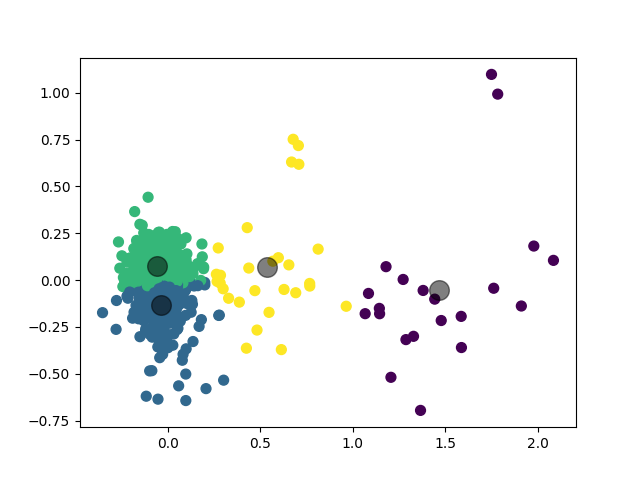
\includegraphics[width=0.7\linewidth]{../../figures/with_background/combined_2mers}
	\caption{A k-means clustering of the combined 2-mers file}
	\label{fig:kmeans0}
\end{figure}

Since we have; methylated/unmethylated, cancer/healthy. Which would result in four groupings of the data. We chose to make 4 clusters of the data.
